% !TEX root = main.tex
\subsection{PGSE-Diffusionskoeffizient}
Im letzten Versuchsteil wird nun der Diffusionskoeffizient bestimmt. Hierfür wird die PGSE-Messmethode (Pulsed gradient spin echo) verwendet um diesen zu bestimmen.
Hierzu wurde die Versuchsanleitung \cite{PGSE} herangenommen.\\
Beim PGSE Experiment wird neben den zwei Pulsen von $90^{\degree}$ und $180^{\degree}$ ein Gradientenfeld angelegt.
Dieses Gradientenfeld wird jedoch nicht die ganze Zeit angelegt, sondern als ein Puls, der nach jedem B$_1$-Puls angelegt wird.
In der folgenden Abbildung \ref{fig:PGSE} kann beobachtet werden, wie ein PGSE-Experiment funktioniert und wie sich die Spins verhalten. 

\begin{figure}[H]
    \centering
    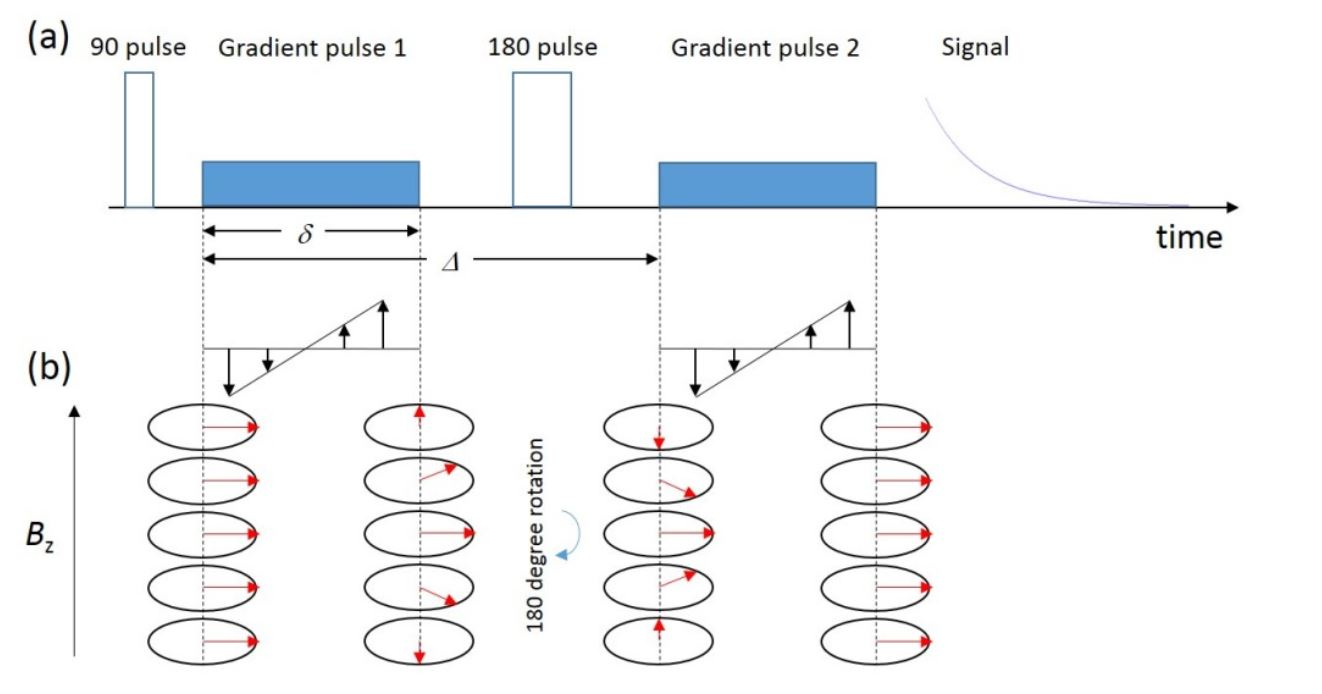
\includegraphics[width=0.8\textwidth]{Abbildungen/PGSE.JPG}
    \caption[Veranschaulichung der PGSE-Messmethode]{Die Abbildung veranschaulicht, wie das PGSE-Experiment funktioniert.
    In der Abbildung (a) sind die zwei B$_1$-Pulse zu beobachten, die vom Hahn-Echo bekannt sind. Nach diesen Pulsen sind zusätzlich zwei Gradientenpulse eingezeichnet. Die Dauer der Gradientenpulse wird als $\delta$ bezeichnet und die Zeit zwischen den beiden Pulsen wird als $\Delta$ bezeichnet.\\
    Die Abbildung (b) zeigt, wie sich die einzelne Spins in der Probe verhalten. Durch das Anlegen eines Gradientenfeldes, stellen sich unterschiedliche Larmorfrequenzen abhängig vom Ort ein. Dadurch präzidieren die Spins unterschiedlich schnell. Durch den $180^{\circ}$-Puls werden die Spins geflippt und durch das anlegen eines gleichen Gradientenfeldes werden die Spins wieder in Phase gebracht.   
    \cite{literaturPGSE}}
    \label{fig:PGSE}
\end{figure}

Wie schon in der Abbildung \ref{fig:PGSE} beschrieben, werden die Spins durch den $90^{\circ}$-Puls als erstes in Phase gebracht. Dies ist links in der unteren Abbildung (b) gezeigt. Durch das anlegen eines Gradientenpulses kommt es zu unterschiedlichen Larmorfrequenzen und somit präzidieren die Spins mit unterschiedlicher Geschwindigkeit.
Wenn zwischen den beiden Gradientenpulsen keine Diffusion stattfindet, so flippt der $180^{\circ}$-Puls die Teilchen. Dies wird in den mittleren zwei Abbildungen gezeigt, wo die Spins von der linken Abbildung in der rechten Abbildung komplett gespiegelt werden. Durch einen zweiten Gradientenpuls werden die spins dann vollständig ausgerichtet. Falls nun keine Diffusion zwischen den zwei Pulsen auftritt, so werden die Spins wieder in Phase gebracht und es entsteht ein Echo,
 wie bei der T$_2$ Messung.
Falls aber zwischen den zwei Phasen eine Bewegung in Gradientenrichtung stattfindet,
so werden nicht alle Spins ausgerichtet. 
Die Bewegung könnte hierbei durch die Diffusion der Teilchen zustande kommen oder kann durch Konvektionsströme in der Flüssigkeit verursacht werden.
Dadurch dass sich die Teilchen aber zwischen dem Gradientenpulsen bewegen, befinden sich diese an unterschiedlichen Orten, falls der Gradientenpuls wieder angelegt wird und somit besitzen die Spins unterschiedliche Larmorfrequenzen im Vergleich zum Anfang.
Somit richten sich die Spins nicht vollständig aus und es entsteht eine modifizierte Echo-Amplitude.
Bei der Betrachtung von dem gemessenen Signalen haben \textit{Stekjskal} und \textit{Tanner} einen Zusammenhang zwischen der normierten Echoamplitude $\frac{\textbf{E}}{\textbf{E}_0}$ und dem Gradienten gefunden. Hierbei wurde festgestellt, dass die Echoamplitude mit einer Exponentialfunktion abfällt. Der Zusammenhang wird hierbei in der folgenden Formel dargestellt:
\begin{align}
    \frac{\textbf{E}}{\textbf{E}_0}&=exp\left(-\gamma^2\delta^2g^2\left(\Delta-\frac{\delta}{3}\right)D_s\right)\\
    D_s&=\text{selbst-Diffusion}\\
    \gamma&= \text{gyromagnetische Moment}\\
    g &= \text{Gradientenpuls-Amplitude}
\end{align}
Indem statt die normierte Amplitude über die Gradienten-Amplitude aufgetragen wird, kann stattdessen $y=ln\left(\frac{\textbf{E}}{\textbf{E}_0}\right)$ über  das Argument der Exponentialfunktion\\
 $x= -\gamma^2\delta^2g^2\left(\Delta-\frac{\delta}{3}\right)$ aufgetragen werden. Somit wird dann im Graphen statt einem exponentiellen Zerfall eine lineare Funktion sichtbar. Diese besitzt die Form $y(x)=-D_sx$ und durch das fitten dieser Funktion wird der selbst Diffusionskoeffizienten ermittelt.       

\begin{figure}[H]
    \centering
    % GNUPLOT: LaTeX picture with Postscript
\begingroup
  % Encoding inside the plot.  In the header of your document, this encoding
  % should to defined, e.g., by using
  % \usepackage[cp1252,<other encodings>]{inputenc}
  \inputencoding{cp1252}%
  \makeatletter
  \providecommand\color[2][]{%
    \GenericError{(gnuplot) \space\space\space\@spaces}{%
      Package color not loaded in conjunction with
      terminal option `colourtext'%
    }{See the gnuplot documentation for explanation.%
    }{Either use 'blacktext' in gnuplot or load the package
      color.sty in LaTeX.}%
    \renewcommand\color[2][]{}%
  }%
  \providecommand\includegraphics[2][]{%
    \GenericError{(gnuplot) \space\space\space\@spaces}{%
      Package graphicx or graphics not loaded%
    }{See the gnuplot documentation for explanation.%
    }{The gnuplot epslatex terminal needs graphicx.sty or graphics.sty.}%
    \renewcommand\includegraphics[2][]{}%
  }%
  \providecommand\rotatebox[2]{#2}%
  \@ifundefined{ifGPcolor}{%
    \newif\ifGPcolor
    \GPcolorfalse
  }{}%
  \@ifundefined{ifGPblacktext}{%
    \newif\ifGPblacktext
    \GPblacktexttrue
  }{}%
  % define a \g@addto@macro without @ in the name:
  \let\gplgaddtomacro\g@addto@macro
  % define empty templates for all commands taking text:
  \gdef\gplbacktext{}%
  \gdef\gplfronttext{}%
  \makeatother
  \ifGPblacktext
    % no textcolor at all
    \def\colorrgb#1{}%
    \def\colorgray#1{}%
  \else
    % gray or color?
    \ifGPcolor
      \def\colorrgb#1{\color[rgb]{#1}}%
      \def\colorgray#1{\color[gray]{#1}}%
      \expandafter\def\csname LTw\endcsname{\color{white}}%
      \expandafter\def\csname LTb\endcsname{\color{black}}%
      \expandafter\def\csname LTa\endcsname{\color{black}}%
      \expandafter\def\csname LT0\endcsname{\color[rgb]{1,0,0}}%
      \expandafter\def\csname LT1\endcsname{\color[rgb]{0,1,0}}%
      \expandafter\def\csname LT2\endcsname{\color[rgb]{0,0,1}}%
      \expandafter\def\csname LT3\endcsname{\color[rgb]{1,0,1}}%
      \expandafter\def\csname LT4\endcsname{\color[rgb]{0,1,1}}%
      \expandafter\def\csname LT5\endcsname{\color[rgb]{1,1,0}}%
      \expandafter\def\csname LT6\endcsname{\color[rgb]{0,0,0}}%
      \expandafter\def\csname LT7\endcsname{\color[rgb]{1,0.3,0}}%
      \expandafter\def\csname LT8\endcsname{\color[rgb]{0.5,0.5,0.5}}%
    \else
      % gray
      \def\colorrgb#1{\color{black}}%
      \def\colorgray#1{\color[gray]{#1}}%
      \expandafter\def\csname LTw\endcsname{\color{white}}%
      \expandafter\def\csname LTb\endcsname{\color{black}}%
      \expandafter\def\csname LTa\endcsname{\color{black}}%
      \expandafter\def\csname LT0\endcsname{\color{black}}%
      \expandafter\def\csname LT1\endcsname{\color{black}}%
      \expandafter\def\csname LT2\endcsname{\color{black}}%
      \expandafter\def\csname LT3\endcsname{\color{black}}%
      \expandafter\def\csname LT4\endcsname{\color{black}}%
      \expandafter\def\csname LT5\endcsname{\color{black}}%
      \expandafter\def\csname LT6\endcsname{\color{black}}%
      \expandafter\def\csname LT7\endcsname{\color{black}}%
      \expandafter\def\csname LT8\endcsname{\color{black}}%
    \fi
  \fi
    \setlength{\unitlength}{0.0500bp}%
    \ifx\gptboxheight\undefined%
      \newlength{\gptboxheight}%
      \newlength{\gptboxwidth}%
      \newsavebox{\gptboxtext}%
    \fi%
    \setlength{\fboxrule}{0.5pt}%
    \setlength{\fboxsep}{1pt}%
\begin{picture}(7200.00,5040.00)%
    \gplgaddtomacro\gplbacktext{%
      \csname LTb\endcsname%%
      \put(814,704){\makebox(0,0)[r]{\strut{}$0.1$}}%
      \put(814,1943){\makebox(0,0)[r]{\strut{}$0.2$}}%
      \put(814,2667){\makebox(0,0)[r]{\strut{}$0.3$}}%
      \put(814,3181){\makebox(0,0)[r]{\strut{}$0.4$}}%
      \put(814,3580){\makebox(0,0)[r]{\strut{}$0.5$}}%
      \put(814,3906){\makebox(0,0)[r]{\strut{}$0.6$}}%
      \put(814,4182){\makebox(0,0)[r]{\strut{}$0.7$}}%
      \put(814,4420){\makebox(0,0)[r]{\strut{}$0.8$}}%
      \put(814,4631){\makebox(0,0)[r]{\strut{}$0.9$}}%
      \put(814,4819){\makebox(0,0)[r]{\strut{}$1$}}%
      \put(946,484){\makebox(0,0){\strut{}$0$}}%
      \put(1922,484){\makebox(0,0){\strut{}$1\times10^{8}$}}%
      \put(2898,484){\makebox(0,0){\strut{}$2\times10^{8}$}}%
      \put(3875,484){\makebox(0,0){\strut{}$3\times10^{8}$}}%
      \put(4851,484){\makebox(0,0){\strut{}$4\times10^{8}$}}%
      \put(5827,484){\makebox(0,0){\strut{}$5\times10^{8}$}}%
      \put(6803,484){\makebox(0,0){\strut{}$6\times10^{8}$}}%
    }%
    \gplgaddtomacro\gplfronttext{%
      \csname LTb\endcsname%%
      \put(198,2761){\rotatebox{-270}{\makebox(0,0){\strut{}Abd\"ampfung $\frac{E}{E_0}$}}}%
      \put(3874,154){\makebox(0,0){\strut{}$\gamma^2 G^2 \delta^2 (\Delta-\frac{\delta}{3})$$\left[\frac{\si{\s}}{\si{\m^2}}\right]$}}%
      \csname LTb\endcsname%%
      \put(5816,4646){\makebox(0,0)[r]{\strut{}Polarisationszeit $\SI{4}{\second}$}}%
      \csname LTb\endcsname%%
      \put(5816,4426){\makebox(0,0)[r]{\strut{}Exponentieller-Fit}}%
    }%
    \gplbacktext
    \put(0,0){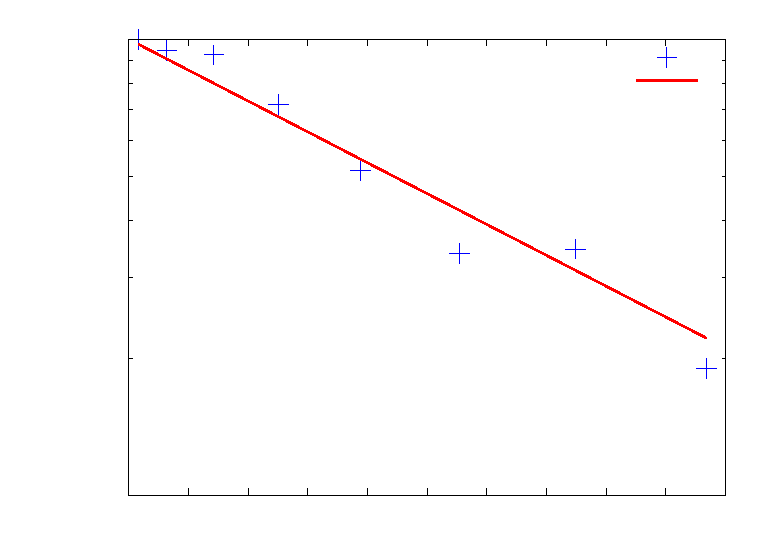
\includegraphics{plots/Diffusion}}%
    \gplfronttext
  \end{picture}%
\endgroup

    \caption[Bestimmung des selbst Diffusionskoeffizienten mithilfe von dem Stejskal-Tanner plot]{\textit{Stejskal-Tanner plot}: Die normierte Amplitude wird Logarhytmisch über $-\gamma^2\delta^2g^2\left(\Delta-\frac{\delta}{3}\right)$ aufgetragen. Hierbei wurde ein Diffusionskoeffizient von $\SI{3,11(26)e-9}{\frac{\m^2}{s}}$ ermittelt}
\end{figure}
 Wenn der ermittelte Wert von $\SI{3,11(26)e-9}{\frac{\m^2}{s}}$ mit dem Literaturwert von $2,299 \cdot 10^{-9}\si{\frac{\m^2}{\s}}$ bei Raumtemperatur ($25^{\circ}$) verglichen wird\cite{Diff}, so wird deutlich, dass die zwei Werte sich in der selben Größenordnung befinden. Es muss aber gesagt werden, dass der Vorfaktor sich um $\pm 1$ unterscheidet. Wenn der Graphe  genauer betrachtet wird, so ist deutlich zu sehen, dass die Werte nicht exakt auf der gefitteten Gerade liegen. Unter anderem könnten die Abweichung dadurch kommen. 
Es gibt nun verschiedene Möglichkeiten, wie diese Messung noch genauer gestaltet werden könnte. Indem unter anderem die Pulslänge varriiert wird, kann diese so angepasst werden, dass sie nicht zu lange ist im Vergleich zur Echozeit. Hinzu kommt noch, dass die Stromstärke groß genug gewählt werden sollte, damit eine ausreichende Dämpfung vorhanden ist.\\
Wenn diese Feinheiten schon justiert oder probiert wurden, so gibt es noch die Option, die Probe an sich noch zu präparieren. Da bei der PGSE-Messung nur die Selbstdiffusion gemessen werden soll, ist darauf zu achten, dass in der Probe keine Konvektionsströme auftreten. Dies kann unteranderem verhindert werden, wenn statt einer Flüssigkeit ein Schwamm genommen wird, der mit der zu untersuchenden Probe getränkt wird. Dadurch treten keine Konvektrionsströme mehr auf und die Bewegung kommen nur durch Diffusion zu stande. Bei dem Schwamm ist darauf zu achten, dass die Poren des Schwammes nicht zu klein sind, damit noch eine Diffusion statt finden kann.\\
Ein weiterer Punkt, warum der Literaturwert von dem ermittelten Wert abweichen könnte, liegt wohl daran, dass die Temperatur am Versuchstag relativ groß war. Durch die zusätzliche Wärme führt dies dazu, dass die Teilchen sich im Gefäß mehr bewegen und dies somit zu einem größeren Diffusionskoeffizienten führt.\\
Eine weitere Sache die zu beachten ist, dass der erste Datenpunkt nicht auf der Geraden liegt. Dies liegt oft an den Konvektionsströmen von der Probe, die vor allem bei größeren Proben auftreten.